\documentclass[12pt]{article}
\usepackage[utf8]{inputenc}
\usepackage[margin=1in]{geometry}
\usepackage{amsmath,amssymb,multicol,enumitem}
\usepackage{pgfplots}
\pgfplotsset{compat=1.17}
\setlength{\parindent}{0pt}
\begin{document}

\fbox{\parbox{0.97\linewidth}{\small\textbf{Final answers} (record here --- graded on the answer; show your work):\\[6pt]1.~\underline{\hspace{1.5cm}}\quad 2.~\underline{\hspace{1.5cm}}\quad 3.~\underline{\hspace{1.5cm}}\quad 4.~\underline{\hspace{1.5cm}}\quad 5.~\underline{\hspace{1.5cm}}}}
\vspace{0.4cm}

\begin{center}{\Large\textbf{Quadratic Functions: Vertex, Max \& Min}}\end{center}
\vspace{0.15cm}

\textbf{Example.}\ For $y=x^{2}-4$ the vertex is $(0,-4)$, which is a \textbf{minimum}. The graph \emph{decreases} for $x<0$ and \emph{increases} for $x>0$.\\[4pt]
\begin{center}
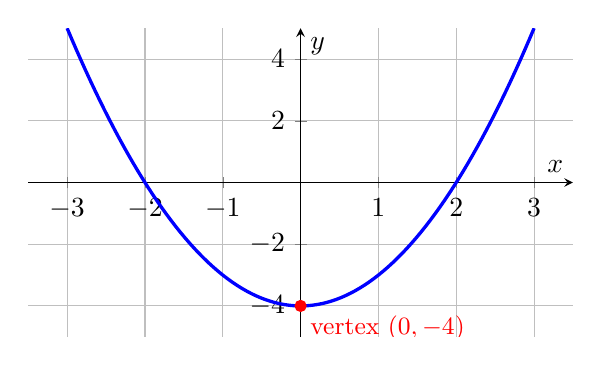
\begin{tikzpicture}
\begin{axis}[axis lines=middle,xlabel=$x$,ylabel=$y$,xmin=-3.5,xmax=3.5,ymin=-5,ymax=5,
  width=8.5cm,height=5.5cm,grid=both,samples=100]
\addplot[very thick,blue,domain=-3:3]{x^2-4};
\addplot[only marks,mark=*,red] coordinates {(0,-4)};
\node[below right,red,font=\small] at (axis cs:0,-4) {vertex $(0,-4)$};
\end{axis}
\end{tikzpicture}
\end{center}
\vspace{0.15cm}\hrule\vspace{0.4cm}

\textbf{Directions: for each function, state max or min, give the vertex, and the increasing / decreasing intervals.}\\[8pt]
\begin{multicols}{2}
\begin{enumerate}[label=\textbf{\arabic*.},itemsep=2.6cm]
\item $y=x^{2}+2$
\item $y=-x^{2}+5$
\item $y=(x-3)^{2}$
\item $y=-(x+1)^{2}-2$
\end{enumerate}
\end{multicols}

\vspace{0.1cm}\hrule\vspace{0.35cm}
\textbf{Challenge}\ (same sheet).\\[6pt]
\begin{enumerate}[label=\textbf{\arabic*.},start=5,itemsep=2.4cm]
\item $y=(x-2)^{2}-9$ --- give the vertex, both intervals, \emph{and} the two $x$-intercepts.
\end{enumerate}

\newpage
\begin{center}{\Large\textbf{Answer Key}}\end{center}
\vspace{0.3cm}
\begin{enumerate}[label=\textbf{\arabic*.}]
\item Min $(0,2)$; decreasing $x<0$, increasing $x>0$
\item Max $(0,5)$; increasing $x<0$, decreasing $x>0$
\item Min $(3,0)$; decreasing $x<3$, increasing $x>3$
\item Max $(-1,-2)$; increasing $x<-1$, decreasing $x>-1$
\item Min $(2,-9)$; decreasing $x<2$, increasing $x>2$; $x$-intercepts $x=-1,\ 5$
\end{enumerate}
\end{document}
